\documentclass[english,usenames,dvipsnames]{beamer}
\usepackage[utf8]{inputenc}
\usepackage[T1]{fontenc}
\usepackage{babel}

\usepackage{enumerate}
\usepackage{algpseudocode}
\usepackage{algorithm}
\usepackage{mathtools}
\usepackage{amssymb}
\usepackage{amsthm}
\usepackage{dsfont}
\usepackage{array}

\usepackage{graphicx}

\usepackage{beamerthemesplit}
\usetheme{Berlin}
\usecolortheme{beaver}

\usefonttheme[onlymath]{serif}

\usepackage{caption}

\usepackage{lmodern}

\usepackage{seqsplit}

\usepackage{bm}
\usepackage{booktabs}

\usepackage{multido}

\usepackage{tikz}
\usepackage{pgfplots}
\pgfplotsset{compat=1.15}
\usepackage{pgfgantt}
\usepackage{appendixnumberbeamer}

\usepackage[absolute,overlay]{textpos}

\usepackage{fontawesome}


%%% For vectors:
\let\vaccent=\v % rename builtin command \v{} to \vaccent{}
\renewcommand{\v}[1]{\ensuremath{\mathbf{#1}}} % for vectors
\newcommand{\gv}[1]{\ensuremath{\mbox{\boldmath$ #1 $}}}
\newcommand{\uv}[1]{\ensuremath{\mathbf{\hat{#1}}}} % for unit vector
\newcommand{\tv}[1]{\ensuremath{\mathbf{\widetilde{#1}}}} % for tilde vector
\let\basetop=\top % rename command \top to \basetop
%\renewcommand{\top}{{}^\basetop \!} % for transpose operation

%%% For general simplified fonctions:
\newcommand{\abs}[1]{\left| #1 \right|} %for absolute value
\newcommand{\avg}[1]{\left< #1 \right>} %for average
\newcommand{\acc}[1]{\left\{ #1 \right\}} %for curly braces
\renewcommand{\det}{\text{det}\hspace{.5pt}} %for determinant
\newcommand{\detpr}[1]{\text{det}\hspace{-2pt}\pr{#1}} %for determinant with braces
\renewcommand{\ln}[1][]{\,\text{ln}\,#1}
\newcommand{\lnpr}[1]{\,\text{ln}\hspace{-1.5pt}\pr{#1}}
\newcommand{\Ln}[1][]{\text{Ln}\,#1}
\newcommand{\tr}[1]{\text{tr}\hspace{-2pt}\pr{#1}} %for trace
\newcommand{\trpr}[1]{\text{tr}\hspace{-2pt}\pr{#1}} %for trace
\newcommand{\diag}[1]{\text{diag}\pr{#1}} %for diagonal
\newcommand{\hc}{\text{h.c.}}

%%% For derivatives:
\let\underdot=\d % rename builtin command \d{} to \underdot{}
\renewcommand{\d}[2]{\cfrac{d #1}{d #2}} % for derivatives
\newcommand{\dx}{\text{d}} % for d in infinitesimal elements
\let\dr=\partial % for "d rond"
\newcommand{\pd}[2]{\frac{\partial #1}{\partial #2}}

%%% For automatic size of delimitors:
\newcommand{\pr}[1]{\left(#1\right)}
\newcommand{\br}[1]{\left[#1\right]}
\newcommand{\cb}[1]{\left\{#1\right\}}
\newcommand{\ceil}[1]{\left\lceil #1 \right\rceil}
\newcommand{\floor}[1]{\left\lfloor #1 \right\rfloor}

%%% For fields and black bold characters
\newcommand{\Id}{\mathds{1}} % For the indicator function in blackboard bold 1
\newcommand{\real}{\mathds{R}} % For the blackboard bold R for real numbers
\newcommand{\Rbb}{\real}
\newcommand{\integer}{\mathds{Z}}
\newcommand{\Zbb}{\integer}
\newcommand{\complex}{\mathds{C}} % For the blackboard bold C for real numbers
\newcommand{\Cbb}{\complex}
% \newcommand{\natural}{\mathds{N}}
\newcommand{\Nbb}{\mathds{N}}
\newcommand{\Fbb}{\mathds{F}}
\newcommand{\Pbb}{\mathds{P}}
\DeclareMathOperator*{\prob}{\Pbb}
\newcommand{\Ebb}{\mathds{E}}
\DeclareMathOperator*{\expectation}{\Ebb}
\newcommand{\Idfunc}[1]{\Id\!\br{#1}}

%%% Raccourcis pour lettres calligraphiques
\newcommand{\A}{\mathcal{A}}
\newcommand{\B}{\mathcal{B}}
\newcommand{\Bb}{{\wb{\mathcal{B}}}}
\renewcommand{\b}{\mathcal{b}}
\newcommand{\bb}{{\wb{\mathcal{b}}}}
\newcommand{\C}{\mathcal{C}}
\newcommand{\D}{\mathcal{D}}
\newcommand{\E}{\mathcal{E}}
\newcommand{\F}{\mathcal{F}}
\newcommand{\G}{\mathcal{G}}
\newcommand{\gluon}{\mathcal{g}}
\renewcommand{\H}{\mathcal{H}}
\newcommand{\K}{\mathcal{K}}
\let\Lslash=\L
\renewcommand{\L}{\mathcal{L}}
\newcommand{\M}{\mathcal{M}}
\newcommand{\m}{\mathcal{m}}
\newcommand{\N}{\mathcal{N}}
\renewcommand{\O}{\mathcal{O}}
\let\parmark=\P
\renewcommand{\P}{\mathcal{P}}
\newcommand{\Q}{{\mathcal{Q}}}
\newcommand{\Qb}{{\wb{\Q}}}
\newcommand{\q}{\mathcal{q}}
\newcommand{\qb}{{\wb{\q}}}
\newcommand{\R}{{\mathcal{R}}}
\renewcommand{\S}{\mathcal{S}}
\newcommand{\T}{\mathcal{T}}
\newcommand{\U}{\mathcal{U}}
\newcommand{\V}{\mathcal{V}}
\newcommand{\W}{\mathcal{W}}
\newcommand{\X}{\mathcal{X}}
\newcommand{\Y}{\mathcal{Y}}
\newcommand{\Z}{\mathcal{Z}}


\newcommand{\softmax}[1]{\text{softmax}\left(#1\right)}

\DeclareMathOperator*{\argmin}{\mathrm{argmin}}
\DeclareMathOperator*{\argmax}{\mathrm{argmax}}


% Tikz settings
\usetikzlibrary{positioning,chains,arrows}
\usetikzlibrary{decorations.pathmorphing}
\usetikzlibrary{decorations.markings}
\usetikzlibrary{decorations.pathreplacing}
\usetikzlibrary{calc}
\usetikzlibrary{arrows.meta}
\usetikzlibrary{bending}
\usetikzlibrary{intersections}
\usetikzlibrary{fadings}
\usetikzlibrary{shapes}

\newcommand{\tikzmark}[1]{\tikz[baseline={(#1.base)},overlay,remember picture] \node[outer sep=0pt, inner sep=0pt] (#1) {\phantom{A}};}
\newcommand{\textbrace}[3]{
	\begin{tikzpicture}[overlay, remember picture,decoration={brace,amplitude=1ex}]
		\draw[decorate,thick] (#1.north east) -- (#2.south east) node[midway, right=0.25cm, align=center] {#3};
	\end{tikzpicture}
}


\tikzstyle{curlybrace}=[-,decorate,decoration={brace,amplitude=2mm,mirror}]
\tikzstyle{curlybracenode}=[midway,below=2mm]

\tikzstyle{tips}=[%
	 btip/.tip = {Latex[length=6, width=3.5]},
	 -btip]
\tikzstyle{neuralnetwork}=[%
	 draw,
	 node distance = 6mm and 24mm,
	 start chain = going below,
	 neuron/.style = {circle, draw,
					  minimum size=25pt, inner sep=0pt,
					  on chain},
	 annot/.style = {text width=4em, align=center,},
	 tips]
\newcommand*{\rnndefaultspacing}{6mm}
\tikzstyle{rnn}=[%
	start chain = going right,
	node distance = \rnndefaultspacing,
	cell/.style = {draw,
					minimum height=3.5em,
					minimum width=1.5em,
					inner sep=1pt,
					on chain},
	tips]



\tikzset{
	invisible/.style={opacity=0},
	visible on/.style={alt={#1{}{invisible}}},
	alt/.code args={<#1>#2#3}{%
		\alt<#1>{\pgfkeysalso{#2}}{\pgfkeysalso{#3}} % \pgfkeysalso doesn't change the path
	},
}



\makeatletter
\DeclareRobustCommand{\rvdots}{%
	\vbox{
		\baselineskip4\p@\lineskiplimit\z@
		\kern-\p@
		\hbox{.}\hbox{.}\hbox{.}
	}}
\makeatother

\graphicspath{{figures/}}



%\usepackage{bibentry}
%\nobibliography*

\usepackage[style=authoryear,maxcitenames=2,uniquelist=false]{biblatex}
\DefineBibliographyExtras{english}{\restorecommand\mkbibnamefamily}
\addbibresource{presentation.bib}
\newcommand\mCite[1]{[\cite{#1}, \citetitle{#1}]}




\beamertemplatenavigationsymbolsempty

\setbeamertemplate{headline}{}

%\setbeamertemplate{footline}[frame number]{}
\usepackage{etoolbox}

\defbeamertemplate{footline}{nonum}{%
    \addtocounter{framenumber}{-1}
}

\BeforeBeginEnvironment{frame}{%
\setbeamertemplate{footline}[frame number]{}
}

\makeatletter
\define@key{beamerframe}{nonum}[true]{%
    \setbeamertemplate{footline}[nonum]%
}
\makeatother


\AtBeginSection[]{
  \begin{frame}[nonum]
  \tableofcontents[currentsection, subsubsectionstyle=hide/hide]
  \end{frame}
}

\AtBeginSubsection[]{
  \begin{frame}[nonum]
	\tableofcontents[currentsection,currentsubsection, subsubsectionstyle=hide/hide]
  \end{frame}
}
\setbeamerfont{subsubsection in toc}{size=\normalsize}

\AtBeginSubsubsection[]{
  \begin{frame}[nonum]
	\frametitle{\insertsubsection}
	\tableofcontents[currentsection,currentsubsection, sectionstyle=hide/hide, subsectionstyle=hide/hide]
  \end{frame}
}


\title[]{Introduction to Deep Learning}
\subtitle{Bootcamp IID 2024}
\author[J. Ngnawé]{Jonas Ngnawé}
\institute{\texttt{\{jonas.ngnawe.1\}@ulaval.ca}}
\date[]{06 mai 2024}


\begin{document}

\begin{frame}[nonum]
\titlepage
\begin{center}
	\vspace{-10mm}
	\begin{columns}
		\begin{column}{0.33\textwidth}
			\includegraphics[width=0.8\textwidth]{iid-bleu.png}
		\end{column}
		\begin{column}{0.33\textwidth}
			\includegraphics[width=0.9\textwidth]{grail.pdf}
		\end{column}
		\begin{column}{0.33\textwidth}
			\hspace{-5mm}
			\includegraphics[width=0.9\textwidth]{ul.pdf}
		\end{column}
	\end{columns}
\end{center}
\end{frame}

\begin{frame}[nonum]
	\tableofcontents[subsubsectionstyle=hide/hide]
\end{frame}

\begin{frame}
	\frametitle{Who Am I?}
	\begin{center}
		\begin{columns}
			\begin{column}{0.4\textwidth}
				\centering
				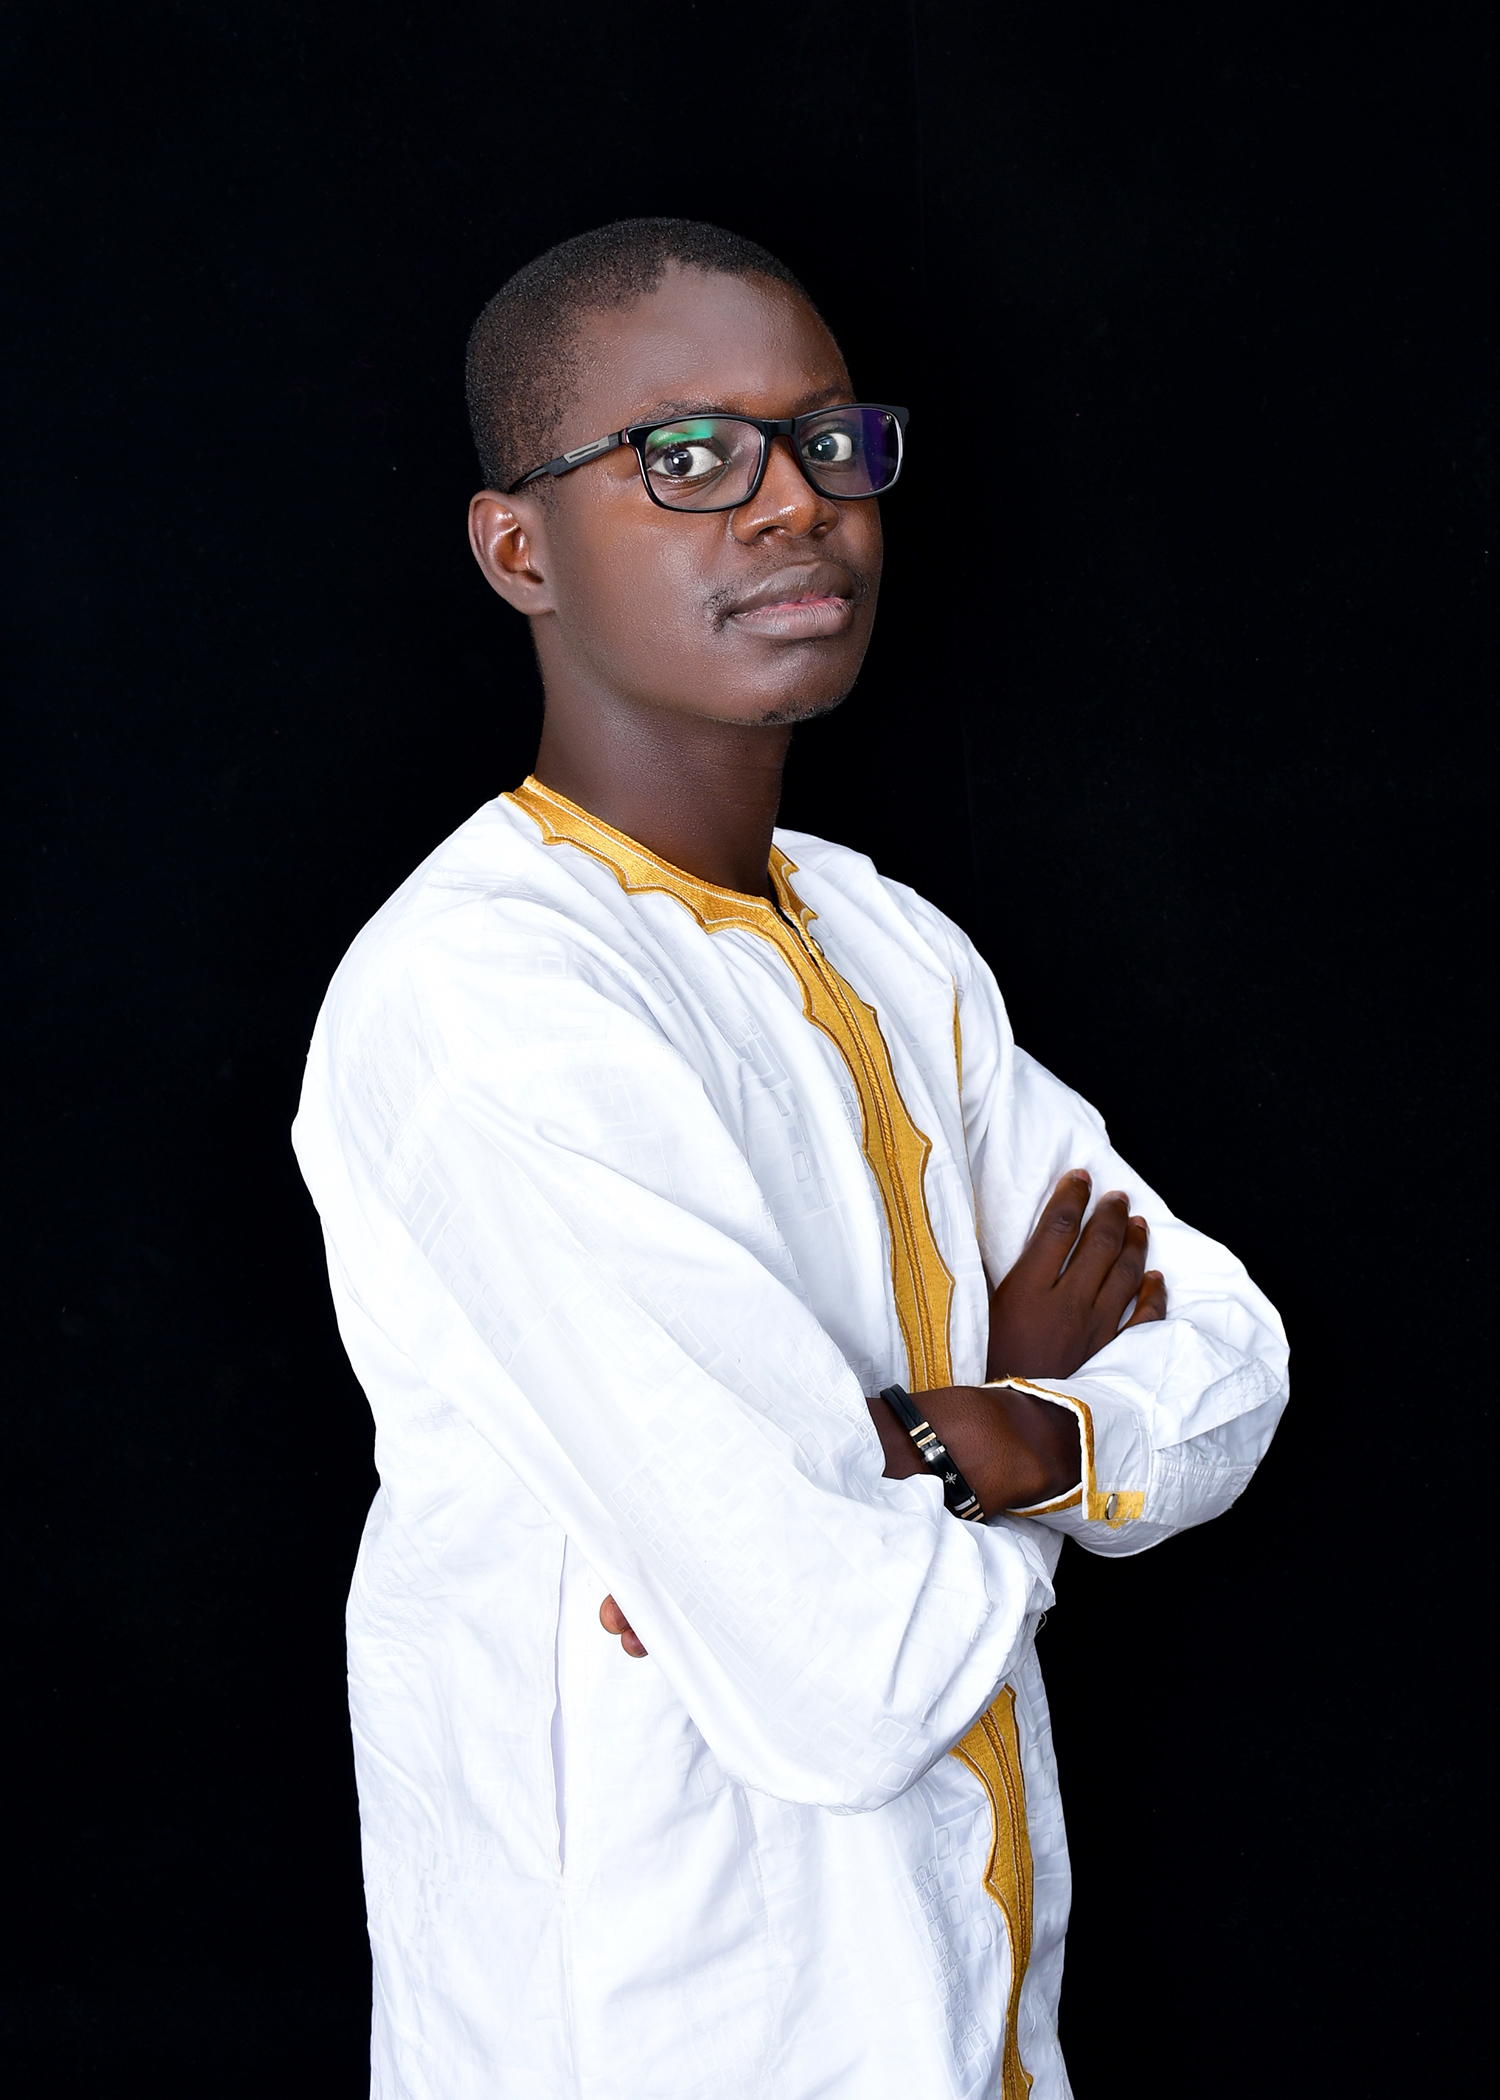
\includegraphics[width=\textwidth]{figures/Jonas.JPG}
			\end{column}
			\begin{column}{0.6\textwidth}
				\textbf{Jonas Ngnawé}\\
				\vspace{1em}
                \includegraphics[height=1em]{ul-notext.pdf} Ph.D. Student at Université Laval (IID \& Mila) \\
				\vspace{0.5em}
				\vspace{1em}
				{\color{NavyBlue} \faLinkedin}~\href{https://www.linkedin.com/in/jonas-ngnawe-bb7712a2/}{jonas-ngnawe-bb7712a2}
			\end{column}
		\end{columns}
	\end{center}
 Slides Credit: Frédérik Paradis, Mathieu Godbout et Alexandre Bouras
\end{frame}


\section{Introduction}

\begin{frame}
	\frametitle{Deep Neural Networks}
	\begin{tikzpicture}[remember picture, overlay]
		\only<1->{
		\node[xshift=1cm,yshift=-1.5cm, anchor=north west, text width=6cm] at (current page.north west){%
		\includegraphics[scale=1]{image_classification}\\\tiny\mCite{Krizhevsky2012ImageNetCW}};}
		\only<2->{
		\node[xshift=-3.5cm, yshift=3.5cm, anchor=south east, text width=5cm] at (current page.south east){%
		\includegraphics[scale=0.25]{google-translate.png}};}
	\end{tikzpicture}
\end{frame}


\begin{frame}
	\frametitle{Computer Vision}
	\framesubtitle{Large Scale Visual Recognition Challenge (LSVRC)}
	{\footnotesize Image classification challenge on the 1,000 image classes of ImageNet}\\[3mm]
	\begin{tikzpicture}
		\node (IMG) {\includegraphics[scale=0.47] {imagenet}};
		\draw[curlybrace] (IMG.south west) + (3.1cm,0mm) coordinate(starthlbrace) -- (starthlbrace -| IMG.south east) node[curlybracenode] {\footnotesize \fontfamily{Times}\selectfont Réseaux profonds};
	\end{tikzpicture}\\[-3mm]
	{\tiny \url{http://www2.ift.ulaval.ca/~pgiguere/cours/DeepLearning/2020/01-Introduction-2020.pdf}}
\end{frame}


\begin{frame}
	\frametitle{Computer Vision}
	\begin{itemize}
		\item<1-> Image classification
		\only<1>{
			\\\includegraphics[scale=1]{image_classification}\\\tiny\mCite{Krizhevsky2012ImageNetCW}
		}
		\item<2-> Object detection
		\only<2>{
			\\\includegraphics[scale=1]{object-detection.png}\\\tiny\mCite{redmon2017yolo9000}
		}
		\item<3-> Image segmentation
		\only<3>{
			\\\includegraphics[scale=0.1]{cityscape.png}\\\tiny\mCite{cordts2016cityscapes}
		}
		\item<4-> Image generation
		\only<4>{
			\\\includegraphics[scale=0.1]{ai_art_prize.jpg}
		}
		\item<5-> etc.
	\end{itemize}
\end{frame}

\begin{frame}
	\frametitle{Natural Language Processing (NLP)}
	\vspace{-5mm}
	\begin{center}
	\includegraphics[scale=0.30,trim={2.5cm 0 2.5cm 1.8cm},clip] {bleu}
	\end{center}
	\vspace{-5mm}
	{\tiny \url{https://paperswithcode.com/sota/machine-translation-on-wmt2014-english-french}}
\end{frame}


\begin{frame}
	\frametitle{Natural Language Processing}
	\begin{itemize}
		\item<1-> Translation
		\only<1>{
			\\\includegraphics[scale=0.25]{google-translate.png}
		}
		\item<2-> Text classification (e.g. topic, sentiment)
		\only<2>{
			\\\includegraphics[scale=0.25]{amazon-review.png}
		}
		\item<3-> Autocorrect
		\only<3>{
			\\\includegraphics[scale=0.1]{autocorrect.jpg}
		}
		\item<4-> Chatbot
		\only<4>{
			\\\includegraphics[scale=0.2]{chatgpt.jpg}
		}
		\item<5-> etc.
	\end{itemize}
\end{frame}
\begin{frame}{History Overview}
	\vspace{-5mm}
	\begin{center}
	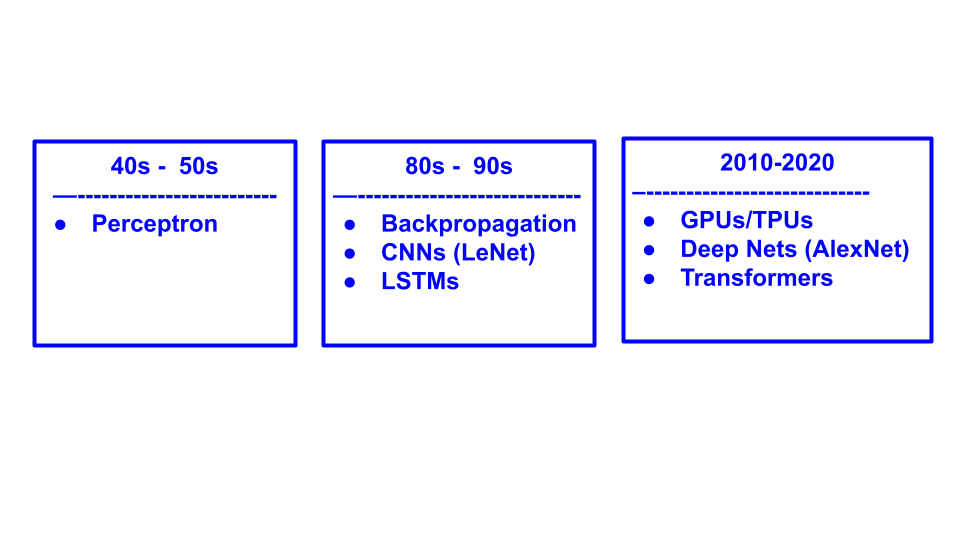
\includegraphics[scale=0.30] {history}
	\end{center}
	\vspace{-5mm}
\end{frame}

\section{Neural Networks}

\begin{frame}
	\frametitle{Machine Learning}

	\begin{center}
		\begin{tikzpicture}[tips]
			\node (DATA) {Dataset $\{(x^{(1)}, y^{(1)}), \dots, (x^{(m)}, y^{(m)})\}$};
			\node[visible on=<2->, anchor=north] (ALGO) at ([yshift=-1.5cm]DATA.south) {Learning algorithm};
			\node[visible on=<3->, anchor=north] (MODEL) at ([yshift=-1.5cm]ALGO.south) {Model};
			\node[visible on=<4->, anchor=east] (IN) at ([xshift=-2cm]MODEL.west) {Input $x$};
			\node[visible on=<5->, anchor=west] (OUT) at ([xshift=2cm]MODEL.east) {Prediction $\hat{y}$};
			\draw[visible on=<2->, -btip] (DATA) -- (ALGO);
			\draw[visible on=<3->, -btip] (ALGO) -- (MODEL);
			\draw[visible on=<4->, -btip] (IN) -- (MODEL);
			\draw[visible on=<5->, -btip] (MODEL) -- (OUT);
		\end{tikzpicture}
	\end{center}
\end{frame}

\begin{frame}
	\frametitle{The Basis of Neural Networks: The Neuron}
	Let $x = (x_1, x_2, \dots, x_n)$ be $n$ features (or variables in statistics).
	\onslide<2->{A neuron computes the following.
		\begin{center}
			\begin{tikzpicture}[neuralnetwork]
				\node[on chain, below=3mm] (I-1) {$x_1$};
				\node[on chain, below=3mm] (I-2) {$x_2$};
				\node[on chain, below=3mm] (DOTS) {$\rvdots$};
				\node[on chain, below=3mm] (I-n) {$x_n$};
				\node[on chain, below right=3mm and 10mm] (BIAS) {$b$};

				\node[circle, draw, minimum size=1.5cm, right=24mm] at (DOTS) (O) {};
				\draw[-] (O.75) coordinate(Otop) -- (O.-75) coordinate(Obottom);
				\path (O.east) -| (Otop) node[pos=.25](sigma) {\LARGE $\sigma$};
				\path (O.west) -| (Otop) node[pos=.25](SUM) {\LARGE $\Sigma$};
				\draw (O.east) -- ([xshift=1cm]O.east);
				\node[visible on=<2>, anchor=west] at ([xshift=1cm]O.east) (EQ) {\LARGE $\displaystyle\sigma\left(\sum_{i=1}^n w_i x_i + b\right)$};
				\node[visible on=<3->, anchor=west] at ([xshift=1cm]O.east) (EQ) {\LARGE $\sigma(w^\top x + b)$};

				\draw (I-1) -- node[pos=0.5, inner sep=1pt, above, sloped] {$w_1$} node[inner sep=1pt, above, pos=0.85] {\tiny+} (O);
				\draw (I-2) -- node[pos=0.5, inner sep=1pt, below, sloped] {$w_2$} node[inner sep=1pt, below, pos=0.85] {\tiny+} (O);
				\draw (I-n) -- node[pos=0.5, inner sep=1pt, below, sloped] {$w_n$} node[inner sep=1pt, below, pos=0.85] {\tiny+} (O);
				\draw (BIAS) -- node[inner sep=3pt, below, pos=0.85] {\tiny+} (O);
			\end{tikzpicture}
		\end{center}
		where $w$ are called the weights of the neuron and $\sigma(\cdot)$ is a non-linear activation function.
	}
\end{frame}


\begin{frame}
	\frametitle{Neural Network}
	\begin{tikzpicture}[neuralnetwork]
		% Draw the input layer nodes
		\node[neuron,draw=none] (I-1) {$x_1$};
		\node[neuron,draw=none] (I-2) {$x_2$};
		\node[neuron,draw=none] (DOTS) {$\rvdots$};
		\node[neuron,draw=none] (I-4) {$x_n$};

		% Draw the 1st hidden layer nodes
		\node[neuron, right=24mm of I-1.center] (H1-1) {};
		\foreach \i in {2,...,4}
		\node[neuron, visible on=<\i->] (H1-\i) {};
		% Draw the 2nd hidden layer nodes
		\node[neuron, above right=6mm and 24mm of H1-2.center, visible on=<5->]  (H2-1)   {};
		\foreach \i in {2,...,3}
		\node[neuron, visible on=<6->] (H2-\i)  {};

		% Draw the output layer node
		\node[neuron, above right=6mm and 24mm of H2-2.center, visible on=<7->]  (O-1)   {$\hat{y}_1$};
		\node[neuron, visible on=<7->] (O-2)  {$\hat{y}_2$};

		% Connect input nodes with hidden nodes and
		%  hiden nodes with output nodes with the output layer
		\foreach \i in {1,2,4}
			\foreach \j in {1,...,4}
			{
			\path (I-\i) edge[visible on=<\j->] (H1-\j);
			}
		\foreach \i in {1,...,4}
		{
			\path (H1-\i) edge[visible on=<5->] (H2-1);
			\foreach \j in {1,...,3}
			{
			\path (H1-\i) edge[visible on=<6->] (H2-\j);
			}
		}
		\foreach \i in {1,...,3}
			\foreach \j in {1,...,2}
			{
			\path (H2-\i) edge[visible on=<7->] (O-\j);
			}

		\draw[curlybrace, visible on=<8->] (starthlbrace -| I-4.west) coordinate(startibrace) -- (startibrace -| I-4.east) node[curlybracenode] {Input};
		\draw[curlybrace, visible on=<8->] (H1-4.south -| H1-4.west) + (0,-1mm) coordinate(starthlbrace) -- (starthlbrace -| H2-3.east) node[curlybracenode] {Hidden layer(s)};
		\draw[curlybrace, visible on=<8->] (starthlbrace -| O-2.west) coordinate(startobrace) -- (startobrace -| O-2.east) coordinate(endobrace) node[curlybracenode] {Output (Prediction)};
		\draw[curlybrace, visible on=<8->] ([yshift=-25pt]starthlbrace) -- ([yshift=-25pt]endobrace) node[curlybracenode] {Number of layers};
	\end{tikzpicture}
    \only<8>{$y=f_L \circ f_{L-1} \circ ... \circ f_2\circ f_1(x)$, $f_\ell=\sigma(W_{\ell-1}f_{\ell-1}+b_{\ell-1})$, $f_0=Id(x)$}
\end{frame}

\begin{frame}
	\frametitle{Activation Functions}
	Given a non-activated output $z = w^\top x + b$, then $\sigma(z) = \dots$
	\begin{itemize}
		\item<2-> $\tanh(z)$
		\begin{center}
			\begin{tikzpicture}
				\begin{axis}[
					xmin=-8, xmax=8,
					ymin=-1.1, ymax=1.1,
					axis lines=center,
					axis on top=true,
					domain=-8:8,
					width=1.5cm,
					height=0.75cm,
					ticks=none,
					scale only axis
					]

					\addplot [mark=none,draw=red, semithick] {tanh(\x)};
				\end{axis}
				\end{tikzpicture}
		\end{center}
		\item<3-> The ReLU function:
		\only<3>{$$\text{ReLU}(z) = \max(0, z)$$}
		\begin{center}
			\begin{tikzpicture}
				\begin{axis}[
					xmin=-2, xmax=2,
					ymin=-0.1, ymax=2,
					axis lines=center,
					domain=-2:2,
					width=1.5cm,
					height=0.75cm,
					ticks=none,
					scale only axis
					]

					\addplot [mark=none,draw=red, semithick] {max(0, \x)};
				\end{axis}
			\end{tikzpicture}
		\end{center}
		\item<4-> The logistic function (also called sigmoid function):
		\only<4>{$$\sigma(z) = \frac{1}{1+\exp(-z)}$$}
		\begin{center}
			\begin{tikzpicture}
			\begin{axis}[
				xmin=-8, xmax=8,
				ymin=-0.05, ymax=1.1,
				axis lines=center,
				axis on top=true,
				domain=-8:8,
				width=1.5cm,
				height=0.75cm,
				ticks=none,
				scale only axis
				]

				\addplot [mark=none,draw=red, semithick] {1 / (1 + exp(-\x))};
			\end{axis}
			\end{tikzpicture}
		\end{center}
		\item<5-> The softmax function:
		\only<5>{$$\softmax{z}_i = \frac{\exp(z_i)}{\sum_{j=1}^m \exp(z_j)}$$ for $z = Wx + b \in \real^m$.}
	\end{itemize}
\end{frame}

\begin{frame}{Other Architectures}
	\begin{center}
		\begin{columns}
			\begin{column}{0.65\textwidth}
				\centering
				\includegraphics[width=\textwidth]{cnn.jpeg}
			\end{column}
			\begin{column}{0.35\textwidth}
				\centering
				\includegraphics[width=\textwidth]{transformer.png}
			\end{column}
		\end{columns}
	\end{center}
\end{frame}

\begin{frame}
	\frametitle{Loss Function}
	Measure of error between a prediction $f(x)$ and a ground truth $y$.\\[2.5mm]
	Goal: minimize the loss function!
	\begin{itemize}
		\item<2-> Mean squared error for regression
		\begin{itemize}
			\item $y, f(x) \in \real$
		\end{itemize}
		$$\L_{\text{MSE}}(f(x), y) = (y - f(x))^2$$
		\item<3-> Cross-entropy loss for classification with $C$ classes ($\Y = \{1, \dots, C\}$)
		\onslide<3->{
		\begin{itemize}
			\item $y \in \Y$
			\item $f(x) = [f(x)_1, \dots, f(x)_C] = \softmax{[z_1, \dots, z_C]}$
		\end{itemize}}
		\onslide<4->{$$\L_{\text{CE}}(f(x), y) = -\log f(x)_y$$}
		\onslide<5>{\begin{center}
			\begin{tikzpicture}
				\begin{axis}[
					xmin=0, xmax=1,
					ymin=0, ymax=4,
					axis lines=center,
					axis on top=true,
					domain=0.01:1,
					width=1.5cm,
					height=1.5cm,
					xtick={0, 1},
					scale only axis
					]

					\addplot [mark=none,draw=red, semithick] {-ln(\x)};
				\end{axis}
				\end{tikzpicture}
		\end{center}}
	\end{itemize}
\end{frame}


\section{Training}

\begin{frame}
	\frametitle{Training Objective}
	Goal: minimize the loss function for all examples (pairs $(x, y)$)!
	\onslide<2->{
		\begin{itemize}
			\item The only thing we control are the parameters $\theta$.
		\end{itemize}
	}
	\begin{align*}
		\onslide<4->{J(\theta) &=} \onslide<3->{\expectation_{(x, y) \in \D}} \L(f(x\only<2->{; \theta}), y) \\
		\onslide<5->{&\approx \frac{1}{N} \sum_{i=1}^N \L(f(x_i; \theta), y_i)}
	\end{align*}
    \onslide<6->{  $$\theta^{*}=\argmin\limits_{\theta \in \Theta} J(\theta)$$}
\end{frame}


\begin{frame}
	\frametitle{Gradient Descent}
	\only<1>{
		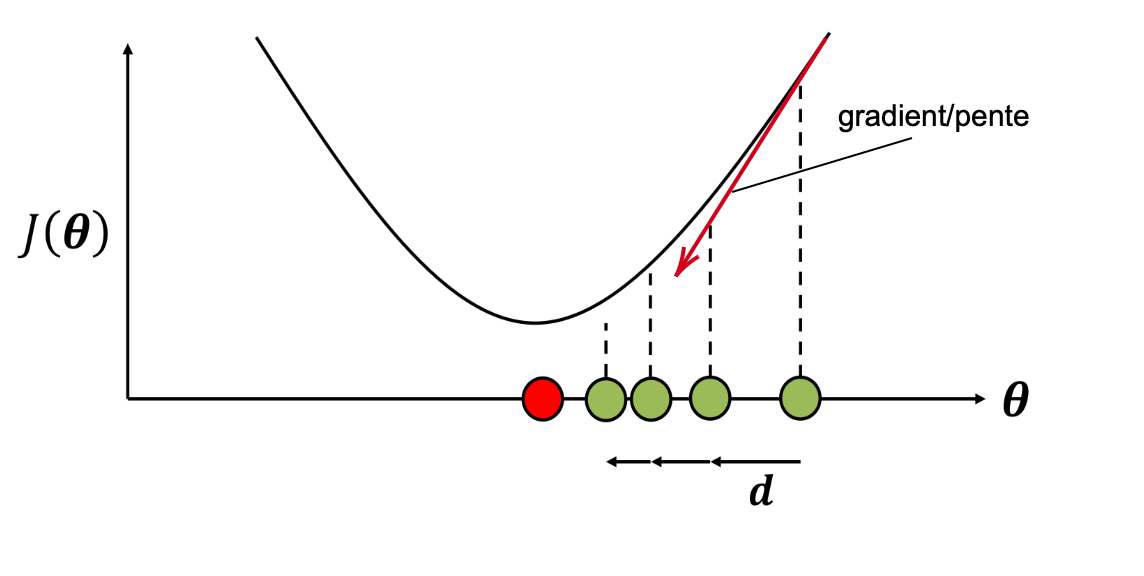
\includegraphics[scale=0.3]{convex-gradient-descent2.png}
		{\tiny From Université Laval GLO-7030 by Ludovic Trottier}
	}
	\only<2>{
		\includegraphics[scale=0.8]{figures/convex-2d-gradient-descent.png}
		{\tiny From Université Laval GLO-7030 by Pascal Germain}
	}
\end{frame}

\begin{frame}
	\frametitle{Gradient Descent For Deep Neural Networks}
	\only<1>{
		\includegraphics[scale=0.2]{convex-not-much-gradient-descent.png}
		{\tiny From Université Laval GLO-7030 by Ludovic Trottier}
	}
	\only<2>{
		\includegraphics[scale=0.5]{hill-descent.pdf}
		{\tiny Adapted by Philippe Giguère for Université Laval GLO-7030 from Standford CS231N}
	}
	\only<3>{
		\includegraphics[scale=0.5]{hidden-hill-descent.pdf}
		{\tiny Adapted by Philippe Giguère for Université Laval GLO-7030 from Standford CS231N}
	}
\end{frame}

\begin{frame}
	\frametitle{Computation of Gradient}
	Using \textbf{"backpropagation"}, we compute the \textbf{partial derivative} of \textbf{the loss} with respect to \textbf{each parameter}. The vector containing all partial derivatives is called the \textbf{gradient}.
	$$d = \nabla_\theta J(\theta) = \left[\frac{\partial J(\theta)}{\partial \theta_1}, \dots, \frac{\partial J(\theta)}{\partial \theta_n}\right]$$
	To update the parameters:
	$$\theta \leftarrow \theta - \epsilon d$$
	$\epsilon$ is called the learning rate.
\end{frame}


\begin{frame}
	\frametitle{Gradient}
	\includegraphics[scale=0.47]{gradient-signal.pdf}\\
	{\tiny Extrait de \url{https://youtu.be/IHZwWFHWa-w} 3Blue1Brown}
\end{frame}


\begin{frame}
	\frametitle{Optimization Algorithms}
	Simplest update rule:
	$$\theta \leftarrow \theta - \epsilon d$$
	Many types exist:
	\begin{itemize}
		\item \textbf{SGD}
		\item SGD with momentum
		\item SGD with momentum Nesterov
		\item Adagrad
		\item RMSprop
		\item \textbf{Adam}
	\end{itemize}
\end{frame}


\begin{frame}
	\frametitle{Training Procedure}
	\begin{center}
		\begin{tikzpicture}[tips]
			\def\myshift{5mm}
			\tikzstyle{noeud}=[draw, rounded corners=1mm, inner sep=2.5mm]
			\node[noeud] (data) {Data};
			\node[noeud, anchor=north] (net) at ([yshift=-\myshift]data.south) {Network};
			\node[noeud, anchor=north] (loss) at ([yshift=-\myshift]net.south) {Loss computation};
			\node[noeud, anchor=north] (backward) at ([yshift=-\myshift]loss.south) {Backpropagation};
			\node[noeud, anchor=north] (optim) at ([yshift=-\myshift]backward.south) {Optimizer step};
			\draw (data) -- (net);
			\draw (net) -- (loss);
			\draw (loss) -- (backward);
			\draw (backward) -- (optim);
			\draw (optim.south) |- ([shift={(-2.5cm, -\myshift)}]optim.south) |- ([shift={(-2.5cm, \myshift)}]data.north) -| (data.north);
		\end{tikzpicture}
	\end{center}
\end{frame}

\begin{frame}
	\frametitle{Training Procedure}
	\begin{center}
		\begin{algorithmic}
			\Procedure{Train}{$f(\cdot;\theta)$, $S$}
				\State \textbf{input:} Neural network $f$ parameterized by $\theta$
				\State \textbf{input:} Dataset $S = \{(x_1, y_1), \dots, (x_N, y_N)\}$
				\onslide<2->{\For{$n$ epochs}
					\onslide<3->{\State Let $S' = S$
					\While{$S' \neq \emptyset$}
						\State Draw a batch $B \subseteq S'$ of $b$ examples.
						\onslide<4->{\State $\ell = \frac{1}{b}\sum_{(x, y) \in B} \mathcal{L}(f(x; \theta), y)$}
						\onslide<5->{\State $d = \nabla_\theta \ell$}
						\onslide<5->{\State Update $\theta$ with $d$ using chosen optimizer}
					\EndWhile}
				\EndFor}
			\EndProcedure
		\end{algorithmic}
	\end{center}
\end{frame}


\section{Overfitting}

\begin{frame}{Neural Networks are Powerful}
	\begin{itemize}
		\item<1-> Universal Approximation Theorem
		\item<2-> ... is a \emph{blessing}!
		\only<2>{
			\\\includegraphics[scale=0.5]{overfitting.png}
		}
		\item<3-> ... and a \emph{curse}!
		\only<3>{
			\\\includegraphics[scale=0.5]{overfitting.png}
		}
		\item<4-> How can we avoid overfitting?
	\end{itemize}
\end{frame}

\begin{frame}
	\frametitle{Regularization}
	Add a penalty term to the loss\footnote{MLE stands for Maximum Likehood Estimation.}:
	$$\L(f(x), y) = \L_{\text{MLE}}(f(x), y) + \lambda\Omega(f)$$
	\begin{itemize}
		\item<2-> L2 regularization: $\Omega(f) = \|\theta\|_2^2$, where $\theta$ are the learneable parameters of the neural network $f$.
		\item<3-> L1 regularization (or LASSO): $\Omega(f) = \|\theta\|_1$
		\item<4-> etc.
	\end{itemize}
\end{frame}


\begin{frame}
	\frametitle{Dropout}
	\includegraphics[scale=0.25]{drop-out.png}
\end{frame}


\begin{frame}
	\frametitle{Early Stopping}
	Extract a validation set $\mathcal{V}$ from the training set. Use it to assess generalization potential.
	\\\includegraphics[scale=0.3]{early_stopping.png}
\end{frame}
\begin{frame}
	\frametitle{More ways to regularize}
	\begin{itemize}
        \item Control the model capacity (e.g.:depth)
	    \item More Data
        \item Data Augmentation
	\end{itemize}
\end{frame}

\begin{frame}
	\frametitle{Deep Learning Libraries}
	\begin{center}
		\begin{columns}
			\begin{column}{0.5\textwidth}
				\includegraphics[width=0.9\textwidth]{tf-logo.pdf}
			\end{column}
			\begin{column}{0.5\textwidth}
				\hspace{-1.5cm}
				{
					\only<1>{
						\setlength{\fboxsep}{6pt}
						\setlength{\fboxrule}{0pt}
						\fbox{\includegraphics[width=1.1\textwidth]{pytorch-logo.pdf}}
					}
					\only<2>{
						\setlength{\fboxsep}{5pt}
						\setlength{\fboxrule}{1pt}
						\fcolorbox{black}{white}{\includegraphics[width=1.1\textwidth]{pytorch-logo.pdf}}
					}
				}
			\end{column}
		\end{columns}
	\end{center}
\end{frame}

\begin{frame}[nonum]
	\begin{center}
		{\Huge PyTorch Demo}
	\end{center}
\end{frame}

\begin{frame}
	\frametitle{Liens de référence}
	\begin{itemize}
		\item Cours GLO-4030/7030 Apprentissage par réseaux de neurones profonds:
		\begin{itemize}
			\item Slides: \url{https://ulaval-damas.github.io/glo4030/}
			\item Laboratoire: \url{https://github.com/ulaval-damas/glo4030-labs}
		\end{itemize}
		\item Vidéos du cours CS231n: \url{https://www.youtube.com/watch?v=vT1JzLTH4G4&list=PLC1qU-LWwrF64f4QKQT-Vg5Wr4qEE1Zxk}
        \item \href{https://karpathy.github.io/2019/04/25/recipe/}{Blogpost: A Recipe for Training Neural Networks. Andrej Karpathy}
		\item Tutoriels et documentation de PyTorch
		\begin{itemize}
			\item \url{https://pytorch.org/tutorials/} (pas tout le temps les meilleures pratiques)
			\item \url{https://pytorch.org/docs/stable/index.html}
		\end{itemize}
		\item Documentation de Poutyne: \url{https://poutyne.org/}
	\end{itemize}

\end{frame}

\begin{frame}[nonum]
	\begin{center}
		{\Huge The End.\\[2cm] Questions?}
	\end{center}
\end{frame}

\begin{frame}[nonum,allowframebreaks]
	\frametitle{Bibliography}
    \printbibliography
\end{frame}

\appendix


\begin{frame}
	\frametitle{Activation Functions}
	Given a non-activated output $z = w^\top x + b$, then $\sigma(z) = \dots$
	\begin{itemize}
		\item<2-> $\tanh(z)$
		\begin{center}
			\begin{tikzpicture}
				\begin{axis}[
					xmin=-8, xmax=8,
					ymin=-1.1, ymax=1.1,
					axis lines=center,
					axis on top=true,
					domain=-8:8,
					width=1.5cm,
					height=0.75cm,
					ticks=none,
					scale only axis
					]

					\addplot [mark=none,draw=red, semithick] {tanh(\x)};
				\end{axis}
				\end{tikzpicture}
		\end{center}
		\item<3-> The ReLU function:
		\only<3>{$$\text{ReLU}(z) = \max(0, z)$$}
		\begin{center}
			\begin{tikzpicture}
				\begin{axis}[
					xmin=-2, xmax=2,
					ymin=-0.1, ymax=2,
					axis lines=center,
					domain=-2:2,
					width=1.5cm,
					height=0.75cm,
					ticks=none,
					scale only axis
					]

					\addplot [mark=none,draw=red, semithick] {max(0, \x)};
				\end{axis}
			\end{tikzpicture}
		\end{center}
		\item<4-> The logistic function (also called sigmoid function):
		\only<4>{$$\sigma(z) = \frac{1}{1+\exp(-z)}$$}
		\begin{center}
			\begin{tikzpicture}
			\begin{axis}[
				xmin=-8, xmax=8,
				ymin=-0.05, ymax=1.1,
				axis lines=center,
				axis on top=true,
				domain=-8:8,
				width=1.5cm,
				height=0.75cm,
				ticks=none,
				scale only axis
				]

				\addplot [mark=none,draw=red, semithick] {1 / (1 + exp(-\x))};
			\end{axis}
			\end{tikzpicture}
		\end{center}
		\item<5-> The softmax function:
		\only<5>{$$\softmax{z}_i = \frac{\exp(z_i)}{\sum_{j=1}^m \exp(z_j)}$$ for $z = Wx + b \in \real^m$.}
		\onslide<6>{\begin{center}
			\begin{tikzpicture}
			\begin{axis}[
				xmin=-8, xmax=8,
				ymin=-8, ymax=8,
				zmin=-0.05, zmax=1.1,
				axis lines=center,
				axis on top=true,
				domain=-8:8,
				width=1.5cm,
				height=1.5cm,
				ticks=none,
				scale only axis,
				view={0}{90},
				legend style={at={(1.05,0.5)}, anchor=west,legend columns=-1},
				]

				\addplot3[surf] {exp(x)/(exp(x) + exp(y))};
				\addlegendentry{$\softmax{z}_1 = \frac{\exp(x)}{\exp(x) + \exp(y)}$ for $z=[x, y]$};
			\end{axis}
			\end{tikzpicture}
		\end{center}}
	\end{itemize}
\end{frame}

\begin{frame}
	\frametitle{Loss Function}
	Measure of error between a prediction $\hat{y} = f(x)$ and a ground truth $y$.\\[2.5mm]
	Goal: minimize the loss function!
	\begin{itemize}
		\item Squared error (SE) for regression:
		$$\L_{\text{SE}}(\hat{y}, y) = (\hat{y} - y)^2$$
		for $\hat{y},y \in \real$.
	\end{itemize}
\end{frame}

\begin{frame}
	\frametitle{Loss Function}
	Measure of error between a prediction $\hat{y} = f(x)$ and a ground truth $y$.\\[2.5mm]
	Goal: minimize the loss function!
	\begin{itemize}
		\item Cross-entropy loss for classification with $C$ classes ($\Y = \{1, \dots, C\}$)
		\onslide<2->{
		\begin{itemize}
			\item $y \in \Y$
			\item $\hat{y} = [\hat{y}_1, \dots, \hat{y}_C] = \softmax{[z_1, \dots, z_C]}$
		\end{itemize}}
		\onslide<3->{
		Based on the cross entropy:
		$$H(q, p) = -\sum_{c \in \Y} {\color{OliveGreen}p(c)} \log {\color{MidnightBlue}q(c)}$$
		}
		\onslide<4->{
		where ${\color{OliveGreen} p(c) = \Id(y = c)}$ and ${\color{MidnightBlue} q(c) = \hat{y}_c}$.} \onslide<5->{This simplifies to:
		$$\L_{\text{CE}}(\hat{y}, y) = -\sum_{c=1}^C {\color{OliveGreen} \Id(y = c)} \log {\color{MidnightBlue} \hat{y}_c} = {\color{RedOrange} -\log \hat{y}_y}$$}
	\end{itemize}
\end{frame}

\begin{frame}
	\frametitle{Convolution Layer}
	\only<1>{\includegraphics[scale=0.5]{cs231n/page68.pdf}}
	\only<2>{\includegraphics[scale=0.5]{cs231n/page69.pdf}}
	\only<3>{\includegraphics[scale=0.5]{cs231n/page70.pdf}}
	\only<4>{\includegraphics[scale=0.5]{cs231n/page71.pdf}}
	\only<5>{\includegraphics[scale=0.5]{cs231n/page72.pdf}}
	\only<6>{\includegraphics[scale=0.5]{cs231n/page73.pdf}}
	\only<7>{\includegraphics[scale=0.5]{cs231n/page74.pdf}}
	\only<8>{\includegraphics[scale=0.5]{cs231n/page75.pdf}}
	\only<9>{\includegraphics[scale=0.5]{cs231n/page76.pdf}}
	\only<10>{\includegraphics[scale=0.5]{cs231n/page77.pdf}}
	\only<11>{\includegraphics[scale=0.5]{cs231n/page78.pdf}}
	\only<12>{\includegraphics[scale=0.5]{cs231n/page79.pdf}}
	\only<13>{\includegraphics[scale=0.5]{cs231n/page80.pdf}}
	\\{\tiny Slides of Fei-Fei Li, Ranjay Krishna, Danfei Xu; Standford CS231n.}
\end{frame}

\begin{frame}
	\frametitle{Other Types of Layers}
	Many types of layers exist. Here is a few.
	\begin{itemize}
		\item Max pooling/averge pooling
		\item Batch normalization
		\item Dropout
	\end{itemize}
\end{frame}

\begin{frame}
	\frametitle{Deep Neural Network Architectures}
	\begin{center}
		\includegraphics[scale=0.75]{AlexNet.pdf}\\
		AlexNet
		\\\tiny\mCite{Krizhevsky2012ImageNetCW}
	\end{center}
\end{frame}

\begin{frame}
	\frametitle{Deep Neural Network Architectures}
	\begin{columns}
		\begin{column}{0.3\textwidth}
			\centering
			\includegraphics[scale=0.37]{VGG.pdf}
			\\VGG
		\end{column}
		\begin{column}{0.4\textwidth}
			\centering
			\includegraphics[scale=0.32]{GoogLeNet.pdf}
			\\GoogLeNet (or Inception)
		\end{column}
		\begin{column}{0.3\textwidth}
			\centering
			\includegraphics[scale=0.37]{ResNet.pdf}
			\\ResNet
		\end{column}
	\end{columns}
	\tiny\mCite{simonyan2014very}\\
	\tiny\mCite{szegedy2015going}\\
	\tiny\mCite{he2016deep}
\end{frame}



\end{document}